%%%%%%%%%%%%%%%%%%%%%%%%%%%%%%%%%%%%%%%%%
% a0poster Landscape Poster
% LaTeX Template
% Version 1.0 (22/06/13)
%
% The a0poster class was created by:
% Gerlinde Kettl and Matthias Weiser (tex@kettl.de)
% 
% This template has been downloaded from:
% http://www.LaTeXTemplates.com
%
% License:
% CC BY-NC-SA 3.0 (http://creativecommons.org/licenses/by-nc-sa/3.0/)
%
%%%%%%%%%%%%%%%%%%%%%%%%%%%%%%%%%%%%%%%%%

%----------------------------------------------------------------------------------------
%	PACKAGES AND OTHER DOCUMENT CONFIGURATIONS
%----------------------------------------------------------------------------------------

\documentclass[a0,landscape]{a0poster}

\usepackage{multicol} % This is so we can have multiple columns of text side-by-side
\columnsep=100pt % This is the amount of white space between the columns in the poster
\columnseprule=3pt % This is the thickness of the black line between the columns in the poster

\usepackage[svgnames]{xcolor} % Specify colors by their 'svgnames', for a full list of all colors available see here: http://www.latextemplates.com/svgnames-colors

\usepackage{times} % Use the times font
%\usepackage{palatino} % Uncomment to use the Palatino font

\usepackage{graphicx} % Required for including images
\graphicspath{{figures/}} % Location of the graphics files
\usepackage{booktabs} % Top and bottom rules for table
\usepackage[font=small,labelfont=bf]{caption} % Required for specifying captions to tables and figures
\usepackage{amsfonts, amsmath, amsthm, amssymb} % For math fonts, symbols and environments
\usepackage{wrapfig} % Allows wrapping text around tables and figures

% For more fonts: see http://www.tug.dk/FontCatalogue/allfonts.html
%\input ArtNouvc.fd
%\newcommand*\initfamily{\usefont{U}{ArtNouvc}{xl}{n}}
%\input Acorn.fd
%\newcommand*\initfamily{\usefont{U}{Acorn}{xl}{n}}
\input Kinigcap.fd
\newcommand*\initfamily{\usefont{U}{Kinigcap}{xl}{n}}
%\input Sanremo.fd
%\newcommand*\initfamily{\usefont{U}{Sanremo}{xl}{n}}
%\input Starburst.fd
%\newcommand*\initfamily{\usefont{U}{Starburst}{xl}{n}}
\definecolor{supercolor}{rgb}{0.1, 0.188, 1}



\begin{document}

%----------------------------------------------------------------------------------------
%	POSTER HEADER 
%----------------------------------------------------------------------------------------

% The header is divided into three boxes:
% The first is 55% wide and houses the title, subtitle, names and university/organization
% The second is 25% wide and houses contact information
% The third is 19% wide and houses a logo for your university/organization or a photo of you
% The widths of these boxes can be easily edited to accommodate your content as you see fit

\begin{minipage}[b]{0.48\linewidth}
\veryHuge \color{NavyBlue} \textbf{PlayCDC - Playing Card Detection} \color{Black}\\ % Title
\Huge\textit{Learning to detect suits and ranks of playing cards}\\[1cm] % Subtitle
\huge \textbf{Frank Gabel \& Daniel Gonzalez}\\ % Author(s)
\huge Ruprecht-Karls-Universit\"at Heidelberg
\\ % University/organization
\end{minipage}
%
\begin{minipage}[b]{0.27\linewidth}
\color{DarkSlateGray}\Large \textbf{Contact Information:}\\
Frank Gabel\\ % Name
Email: \texttt{frank.gabel@med.uni-heidelberg.de}\
\\\\
Daniel Gonzalez \\
%Phone: +1 (000) 111 1111\\ % Phone number
Email: \texttt{d.gonzalez@stud.uni-heidelberg.de}\\ % Email address
\end{minipage}
%
\begin{minipage}[b]{0.45\linewidth}


\includegraphics[width=30cm]{playcdc.png} \vspace{3cm}% Logo or a photo of you, adjust its dimensions here
\end{minipage}

\vspace{1cm} % A bit of extra whitespace between the header and poster content

%----------------------------------------------------------------------------------------

\begin{multicols}{3} % This is how many columns your poster will be broken into, a poster with many figures may benefit from less columns whereas a text-heavy poster benefits from more

%----------------------------------------------------------------------------------------
%	ABSTRACT
%----------------------------------------------------------------------------------------

\color{Navy} % Navy color for the abstract

\centering\section*{Abstract}
\raggedright	
\Large
With the capabilities of upcoming small video capturing devices in, for example, smart contact lenses with built-in cameras, whole new ways of cheating in cardgames emerge. In order to help facilitate these cheating endeavours, we implement an algorithm that detects the suits and ranks of playing cards in the field of view of a camera using the latest iteration of the YOLO object recognition algorithm.


%----------------------------------------------------------------------------------------
%	INTRODUCTION
%----------------------------------------------------------------------------------------
\color{DarkSlateGray} % DarkSlateGray color for the rest of the content


\large

%A big topic in computer vision is the search of methods that are, given a query image, capable of answering questions like: What is present in an image? Is there a particular object in it? Where exactly in the image is this object located?
%Object detection deals with detecting instances of semantic objects of a certain class (such as humans, buildings, or cars) in digital images and videos. Typically, object detection deals with two sub-taks: \textbf{object localization} using bounding boxes and \textbf{multiclass object classification} within said bounding boxes.
%In this project, we implement the YOLOv3 object detection algorithm.

%----------------------------------------------------------------------------------------
%	OBJECTIVES
%----------------------------------------------------------------------------------------

\color{DarkSlateGray} % DarkSlateGray color for the rest of the content

\section*{Main Objectives}
The objectives of this project are summarized as follows:

\begin{description}

\item[Create a general dataset] of a standard, 52-card deck of playing cards  in different poses, brightness situations and blurring levels annotated with bounding boxes around the ranks and suits and corresponding class information.
\item[Train an object detection algorithm] on these synthesized data that performs bounding box localization and regression for classification. In particular, we train  the latest iteration of the YOLO object detection algorithm \cite{DBLP:journals/corr/abs-1804-02767} end-to-end.
\item[Evaluate the algorithm on a hold-out validation dataset] covering all classes. As a performance metric, mean Average Precision (mAP) is used.
\item[Deploy the model on a smartphone camera] as a proof of concept.

\end{description}


%----------------------------------------------------------------------------------------
%	MATERIALS AND METHODS
%----------------------------------------------------------------------------------------

\section*{Methods}
\subsection*{Dataset creation pipeline}
The dataset was created in mainly 2 big steps. \\
\begin{description}
\item[Prepare raw card images] We took two photos for each card of a deck of 52 cards, manually crop the cards to a selection and rescale the result by 900$\times$600 pixels using GIMP.
After this, we detect the convex hulls of the cards suits and ranks using the Python libraries SciPy and OpenCV.  \\
\item[Synthesize a general dataset]  First, we pasted the images in canvances provided by DTD \cite{cimpoi14describing} in order to have different textures around the images.
In order to generate a considerable amount of training data, we apply different transformations to each image (blurring, sharpening, change of lighting, rotation, small shears).
As convex hull information changes during operations such as rotation, we used the Python library imgaug to keep track of the correct coordinates at all times. \\
The final datasets consisted of up to 25000 images.
\end{description}



% IMAGES
% \centering\vspace{1cm}
 %	\begin{minipage}[b]{0.16\textwidth}
  % 		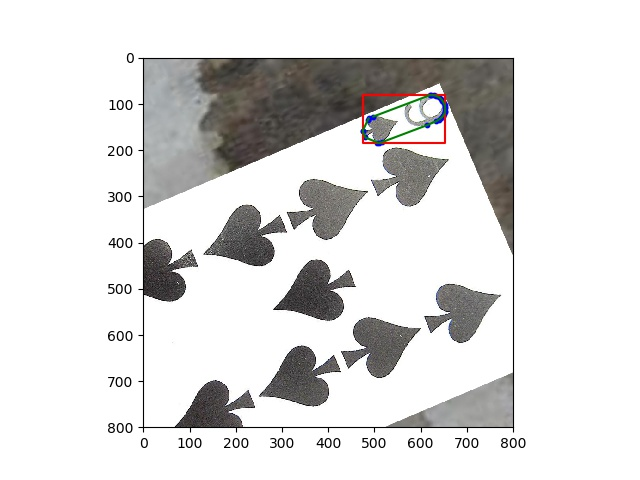
\includegraphics[width=\textwidth]{7-full}
%		\captionof{figure}{\color{Green} Figure caption}
% 	 \end{minipage}
% \hspace{2cm}
% 	\begin{minipage}[b]{0.12\textwidth}
 %  		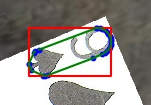
\includegraphics[width=\textwidth]{7}
%		\captionof{figure}{\color{Green} Figure caption}
% 	\end{minipage}\vspace{1cm}

\vspace{1cm}
\begin{minipage}[b]{0.27\textwidth}
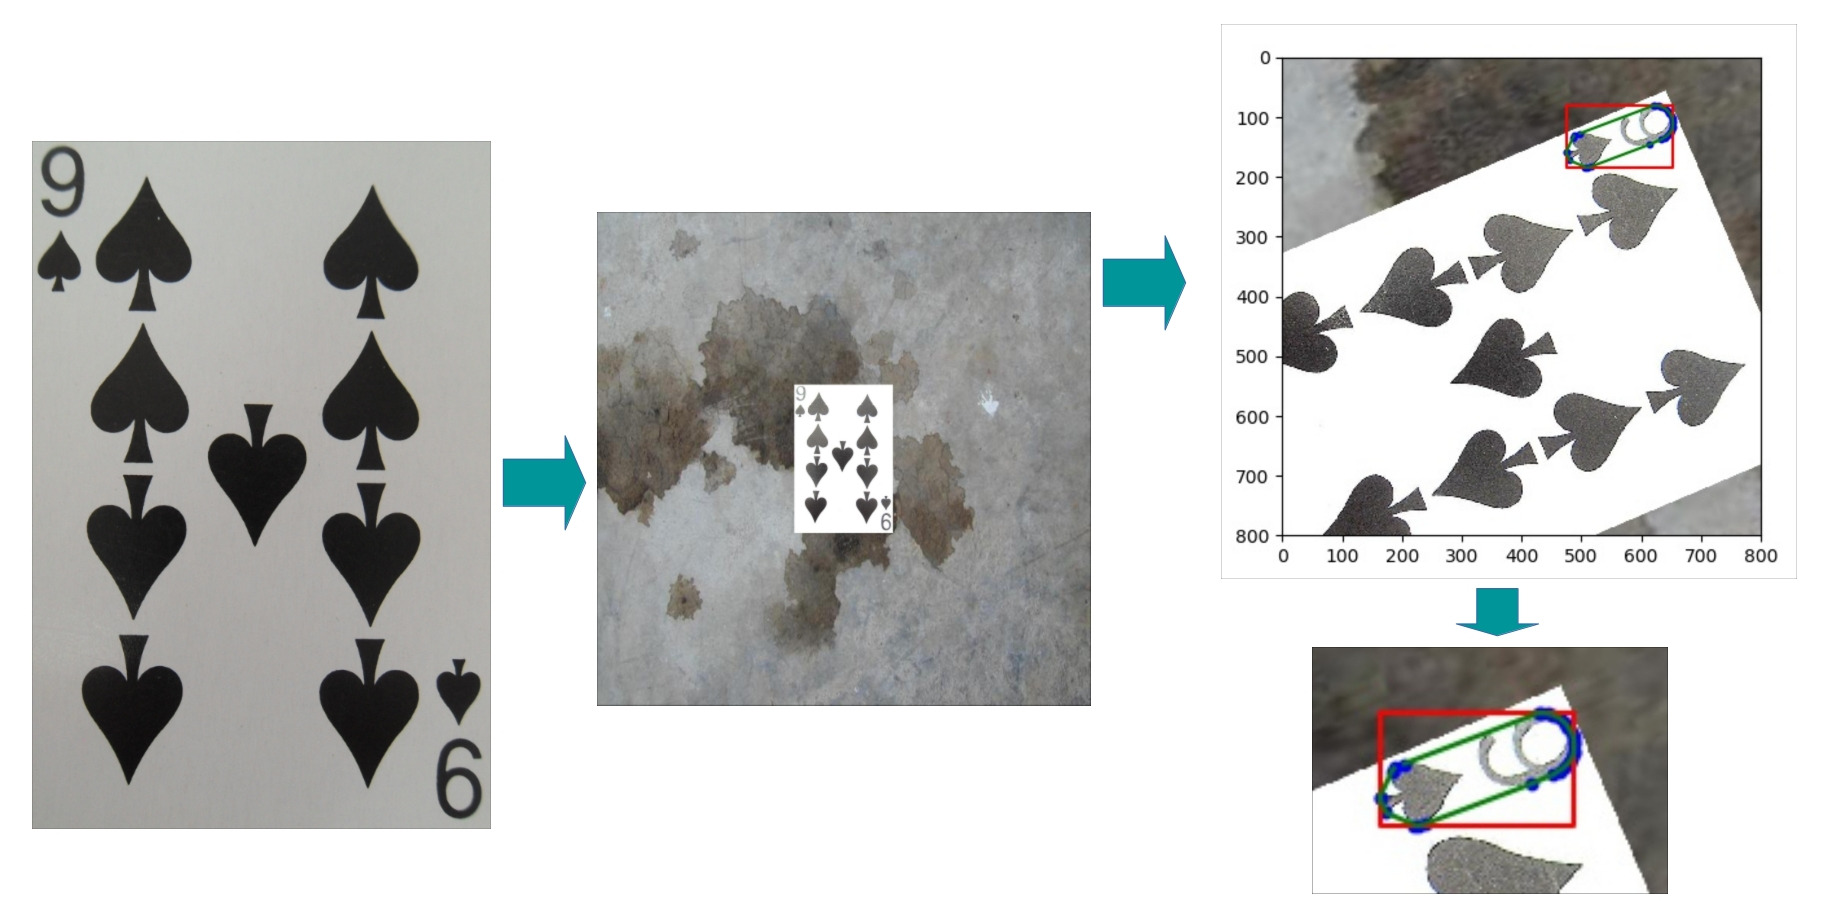
\includegraphics[width=\textwidth]{7-p}
\captionof{figure}{The dataset creation pipeline: paste photographs of images onto textures and apply random transformations to both images and corresponding convex hulls/bounding boxes}
\end{minipage}
%\begin{center}\vspace{1cm}
%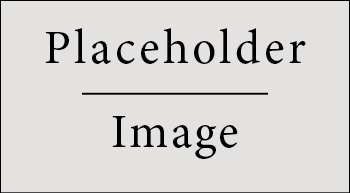
\includegraphics[width=0.5\linewidth]{placeholder}
%\captionof{figure}{\color{Green} Figure caption}
%\end{center}\vspace{1cm}
%------------------------------------------------

\subsection*{The YOLO approach to object detection}
The YOLO approach works by modelling detection as a \textbf{regression problem}, where the image is divided into an $S\times S$ grid and for each grid cell \textbf{$B$ bounding boxes} are predicted along with the \textbf{confidence} and \textbf{$C$ class probabilities} for these boxes. \\
These predictions are performed simultaneously by a single CNN.
\subsubsection*{tiny YOLO-v3}

The particular architecture we used for training on our dataset is \textbf{tiny YOLOv3} which essentially is a smaller version of YOLO for constrained environments.
\begin{center}\vspace{0cm}
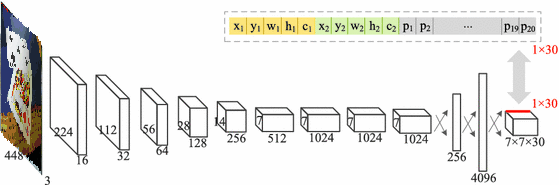
\includegraphics[width=0.7\linewidth]{tinyyolo}
\captionof{figure}{tiny YOLO-v3 feature extractor}
\end{center}\vspace{0cm}

%\subsection*{Evaluation strategy}
%The evaluation of object detection algorithms is not easy as two tasks need to be evaluated: \textbf{localization} and \textbf{classification}.
%Therefore, often, mean Average Precision (mAP) is used in literature where mean classification performance (as measured by the precision) is averaged across predictions using different IOU thresholds.


%----------------------------------------------------------------------------------------
%	RESULTS 
%----------------------------------------------------------------------------------------

\section*{Results}


We consecutively trained on increasingly general datasets, starting with cards pasted on a white canvas to cards pasted on varying textures as backgrounds. This strategy improved generalisability on random test images, but also decreased the test mAP slightly as the tasks became "harder". Deploying tinyYOLO on a webcam using a (rather slow) GPU (GeForce GTX 960M) resulted in about 35 FPS depending on brightness levels which is essentially real-time.
\begin{wrapfigure}{r}{0.2\textwidth}

    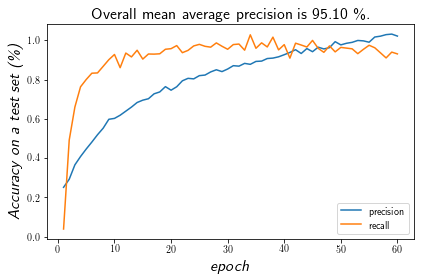
\includegraphics[width=0.22\textwidth]{traindev}



    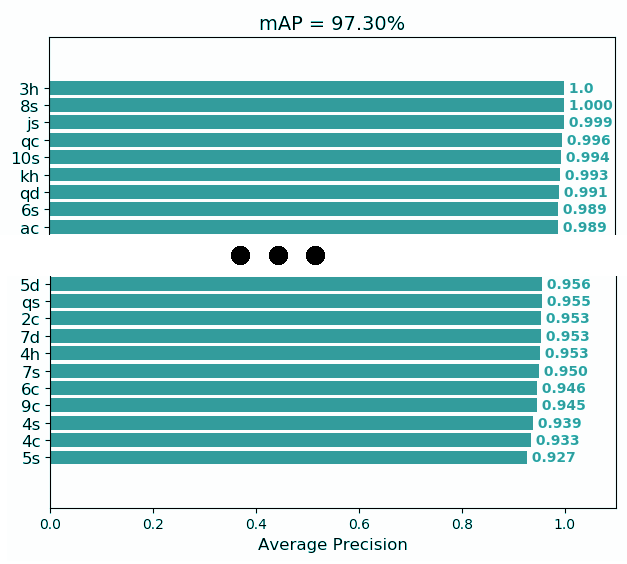
\includegraphics[width=0.22\textwidth]{mAP}
\hspace*{2cm}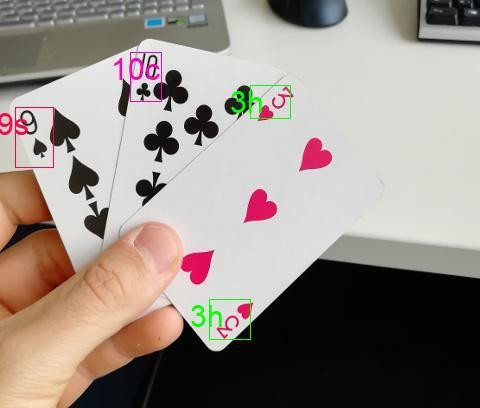
\includegraphics[width=0.18\textwidth]{ex}

  \caption{Training performance on holdout datasets across epochs (top) and performance of the final trained model across different classes (mid), cherry-picked test result on a randomly taken photo (bottom)}
\end{wrapfigure}
For the most general dataset, we reached a mAP of \textbf{97.30\%}. Using a dataset consisting of "easier" transformations (in particular, less blurring) resulted in a mAP of \textbf{99.11\%}, but did considerably worse on random images of cards not from the same deck.




%----------------------------------------------------------------------------------------
%	CONCLUSIONS
%----------------------------------------------------------------------------------------


\section*{Conclusions}

\begin{itemize}
\item Using an artificially created dataset, we achieve a mAP score of 97.30\% on a holdout dataset.
\item The task of object detection on ranks/suits of playing cards appears to be easy as it can be thought of as 2D rather than 3D.

\end{itemize}



\color{DarkSlateGray} % Set the color back to DarkSlateGray for the rest of the content


\nocite{*} % Print all references regardless of whether they were cited in the poster or not
\bibliographystyle{acm} % Plain referencing style
\footnotesize
\bibliography{sample} % Use the example bibliography file sample.bib


%----------------------------------------------------------------------------------------

\end{multicols}
\end{document}